\begin{figure}
	\begin{tabular}{c c}
		\subfloat[original frame]{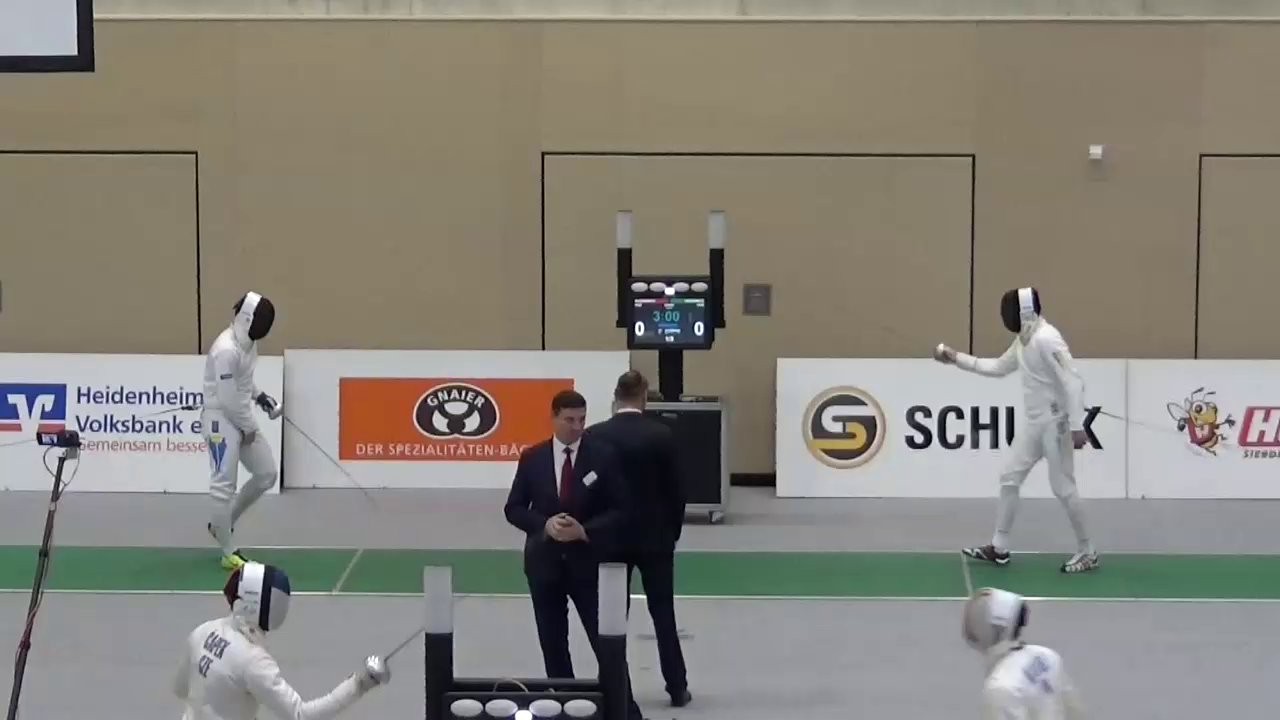
\includegraphics[width = 0.45\columnwidth]{images/fencing/original_frame.png}}    & 
		\subfloat[People area masking]{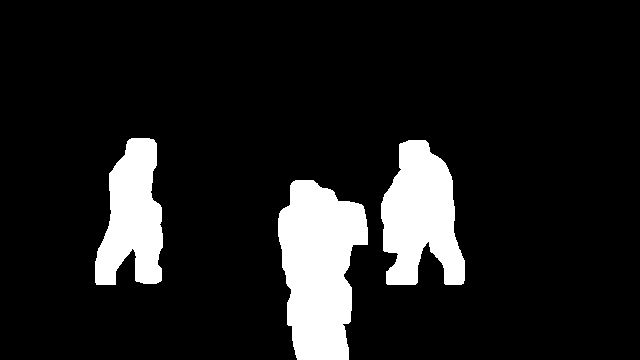
\includegraphics[width = 0.45\columnwidth]{images/fencing/masked_frame.png}} \\
		\subfloat[Optical flow]{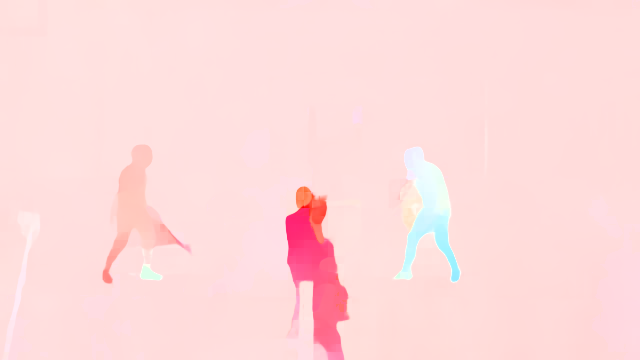
\includegraphics[width = 0.45\columnwidth]{images/fencing/flow_frame.png}}          &
		\subfloat[Person area inpainting]{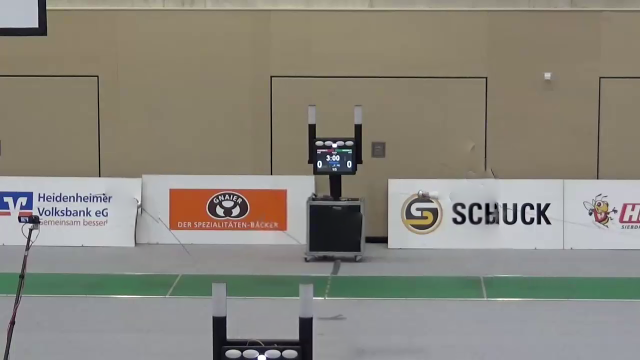
\includegraphics[width = 0.45\columnwidth]{images/fencing/no-person-frame.png}}
	\end{tabular}
	\caption{process until the person area is inpainted}
	\label{fig:inpaint}
\end{figure}

The framework proposed in this study can be divided into three main stages. In the first stage, a panoramic image is generated from a video camera image; in the second stage, the player's posture coordinates and absolute coordinates on the court are estimated from the panoramic image. In the second stage, we estimate the posture coordinates and the absolute coordinates of the player on the court from the panoramic images. In the last stage, we analyze and visualize the obtained skeletal and positional information of the player by dimensional compression and clustering. The details of each element are described below.

\subsection{Generation of panoramic images}
Since it is strategically useful to know where the players are on the court, it is useful to generate panoramic images showing the entire court. In addition, the position of the players on the pitch can be estimated from the panoramic image by using person detection, so that the positional information of the players can be obtained not only visually but also numerically.

\subsection{extraction of person region}

Usually, panoramic background images are generated using images of only stationary objects, so to use conventional methods, moving objects, i.e., humans, must be eliminated in each frame, and the eliminated areas must be complemented in some way. In this study, this is done in two steps.
For the extraction of human regions, we use segmentation with HR-NET\cite{SunXLW19}, and label each pixel of each frame as human region (=1) or not human region (=0). As a post-processing step, we perform smoothing operations in the vertical, horizontal, and temporal directions to mask the human region more reliably in each frame. \ref{fig:inpaint}(b) shows the masking of the person area after post-processing.

\subsection{inpainting of human area}
The masked human region is inpainted by calculating the optical flow in the front-back direction based on the Flow-edge Guided Video Completion\cite{Gao2020} method. 
% The result is an unattended video where the person is seamlessly removed from the video. %Figure \ref{sec:inpaint}(c) shows the result of visualizing the optical flow and (d) shows the result after inpainting the human region.

% \subsection{selection of keyframe image}
% The unattended image generated above does not contain any human, so there are almost no moving objects, which is suitable for panoramic images. However, the time complexity of the conventional Image Stitching method \cite{brown2007automatic} is $O(4N^3)$ when $N$ is the number of frames. It would take an enormous amount of time. Therefore, we selected keyframes to create a high-quality panoramic video that captures the entire court even with a small number of frames.

% \begin{figure}
% \begin{tabular}{c}
% \subfloat{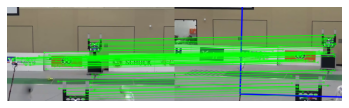
\includegraphics[width = \linewidth]{images/fencing/homography.png}} &
% \end{tabular}
% \caption{SIFT feature matching with RANSAC method}
% \label{homo}
% \end{figure}

% First, the estimated projection matrices of the first frame of the video and the other frames are flattened and used as feature vectors. To estimate the projection matrix, we compute the SIFT feature \cite{lowe2004distinctive} in the image and use keypoint matching with the RANSAC method \cite{fischler1981random}. Figure \ref{homo} shows the result of keypoint matching between two frames as an example.

% The feature vectors are reduced to two dimensions by Principal Component Analysis (PCA)\cite{wold1987principal} and T-Stributed Stochastic Neighbor Embeddings (T-SNE)\cite{maaten2008 Figure \cite{wold1987principal} and T-distributed Stochastic Neighbor Embeddings (T-SNE)\cite{maaten2008 visualizing} show the dimensional compression to two dimensions in Figure \cite{homography_viz}(d),(e). In Figure \ref{homography_viz}, the frames (a) Left, (b) Middle, and (c) Right correspond to the colored points in the scatter plot, and are distributed along the x-axis, indicating that the left and right information is concentrated in the first principal component. Using this phenomenon, we sample 10 frames that are distributed as evenly as possible from only the first principal component of the dimensionally compressed feature vector using PCA, and use them to paste the images together.

% \begin{figure}
% \begin{tabular}{ccc}
% \subfloat[Left]{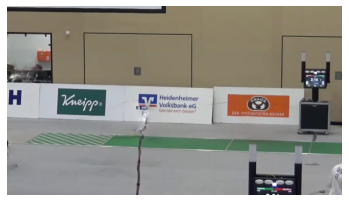
\includegraphics[width = 0.3\linewidth]{images/fencing/left.png}} &
% \subfloat[Middle]{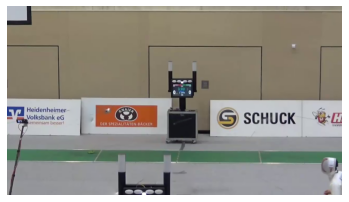
\includegraphics[width = 0.3\linewidth]{images/fencing/middle.png}} &
% \subfloat[Right]{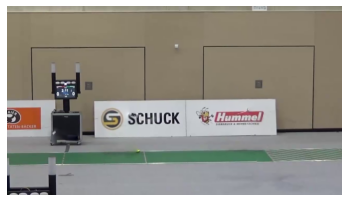
\includegraphics[width = 0.3\linewidth]{images/fencing/right.png}}
% \\end{tabular}
% \begin{tabular}{cc}
% \subfloat[T-SNE Plot]{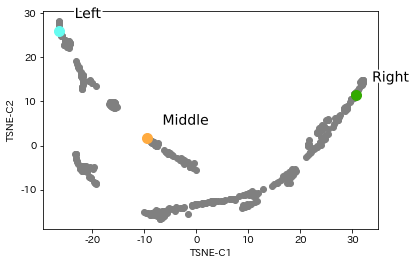
\includegraphics[width = 0.5\linewidth]{images/fencing/tsne.png}}
% {\subfloat[PCA Plot]{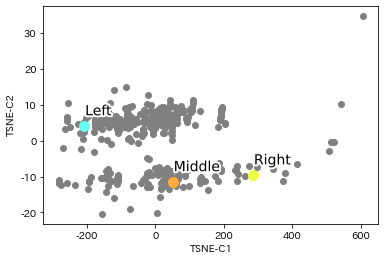
\includegraphics[width = 0.5\linewidth]{images/fencing/pca.png}}
% \end{tabular}
% \caption{A scatterplot of feature vectors dimensionally compressed by (d) T-SNE and (e) PCA. Each point represents a single frame.}
% \label{homography_viz}
% \end{figure}

% \subsection{connecting keyframe images}\label{connecting keyframe images}
% Generate a single unattended background panorama by stitching together keyframe images using the images selected in \ref{select keyframe images}. For stitching, we use the Image Stitcher Class in OpenCV\cite{opencv_library}, which has a full pipeline of image registration (feature matching, wave correction, etc.) and image composition (warping, blending, etc.).

% To remove noise from unattended background panoramas, the process of \ref{select keyframe images}is performed several times to generate several slightly different unattended background panoramas and apply a pixel-wise median filter. Figure \ref{panos}(a) shows the result.

% To create panoramic images from the unattended background panoramas, we compute the projection matrix by matching the SIFT features with the RANSAC method on the unattended background panoramas and each frame. The player can be overlaid on the unattended panorama by applying a matrix transformation using the projection matrix calculated above to the bounding box of the player detected by the method described in \ref{Detecting and Tracking the Player}. Figure \ref{panos}(c) shows how this process is applied.

% %\begin{figure}
% %\begin{tabular}{c}
% %\subfloat[Example of selected keyframe images]{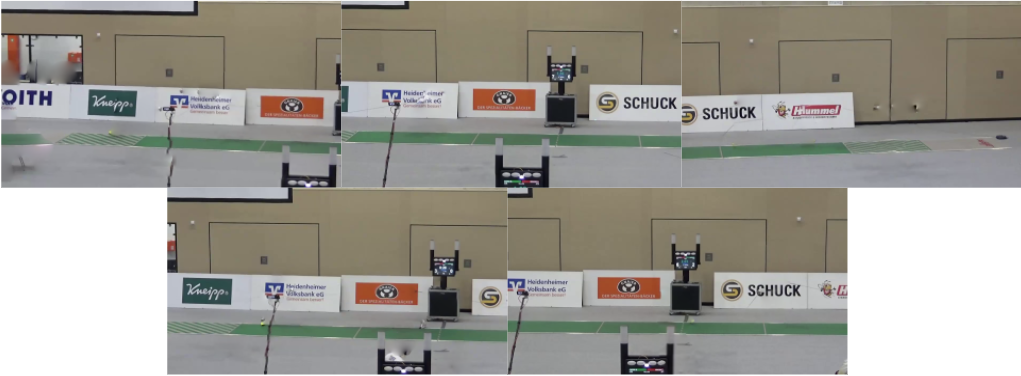
\includegraphics[height = 20mm]{images/fencing/pre-pano.png}}
% %\subfloat[Unattended panoramic image]{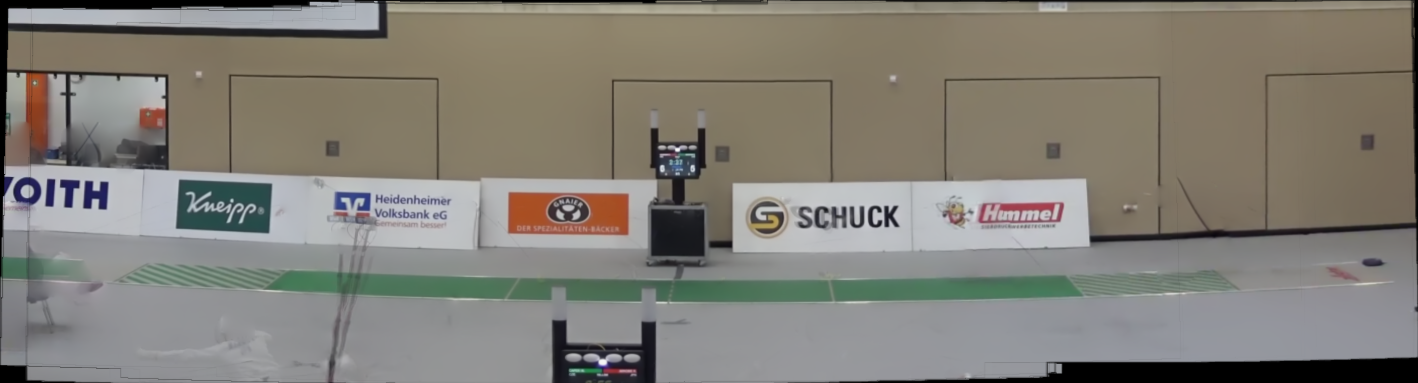
\includegraphics[width = \linewidth]{images/fencing/panorame_no_people.png}}
% % \end{tabular}
% %\caption{}
% %\end{figure}

% \subsection{extraction of skeletal and positional information}}
% By applying the existing object detection and posture estimation techniques to the panoramic video, we can easily obtain the skeletal and positional information of the player. The details of the method are described below.

% \subsection{Detect and track the corresponding player}\label{Detect and track the corresponding player}
% To detect and track the players, we use FairMOT\cite{zhang2020fair}. FairMOT solves the problems of traditional multi-object tracking (MOT) methods by using a single-shot deep neural network without anchors. FairMOT solves the problems of conventional multi-object tracking (MOT) methods by using a single-shot deep neural network without anchors, and is SoTA in terms of both tracking accuracy and inference speed.

% In addition to the player in question, there are referees and players from other games in the match video, so it is necessary to sort them out. To do so, we first manually annotate the unattended panoramic video with the areas of the court where the players in the game should be.
% If the detected person is out of the area, the person is removed as noise. If the person is not out of the area, the person is used as the corresponding player in the overlay created through the process of \ref{connecting keyframe images}. In Figure \ref{panos}(b), the players that are out of the region are shown as "DELETE" and the players that are not out of the region are shown as "KEEP". When only one player was detected for the overlay, linear completion was used. When three or more players were detected, players were selected using bipartite matching \cite{kuhn1955hungarian}, a Hungarian algorithm that treats skeletal information as a graph.

% \subsection{extraction of skeletal and location information}
% PifPaf\cite{Kreiss_2019}is used to obtain skeletal information for the bounding boxes of the relevant players detected by \ref{Detect and track relevant players}. The skeletal information obtained using this pose estimator is shown in Figure \ref{panos}(d).


% %\begin{figure}
% %\begin{tabular}{c}
% %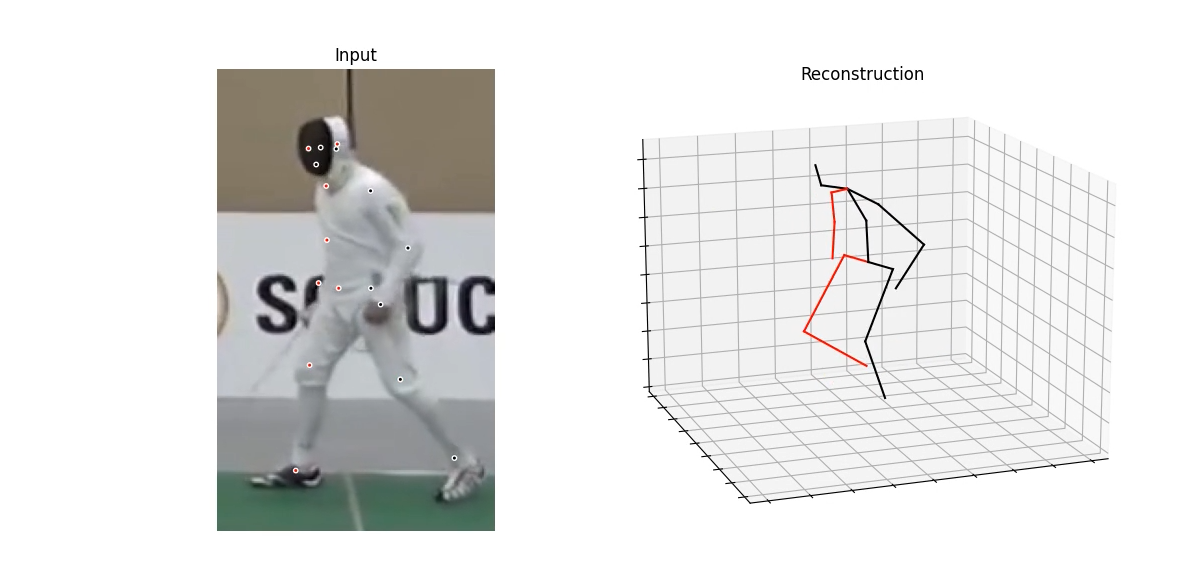
\includegraphics[width = 0.8\linewidth]{images/fencing/videopose.png}
% %\end{tabular}
% %\caption{Pose Estimation with Video Pose}
% %\label{videopose}
% %\label{panos}
% %\end{figure}


% \begin{figure}
% \begin{tabular}{c}
% \subfloat[unattended panorama image]{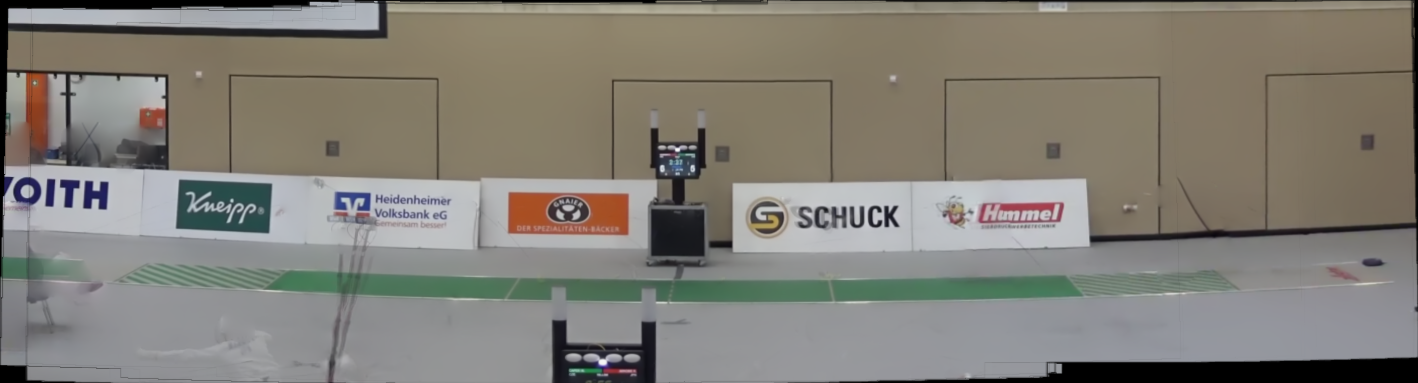
\includegraphics[width = \linewidth]{images/fencing/panorame_no_people.png}}
% \subfloat[Area of the court in the unattended panoramic image]{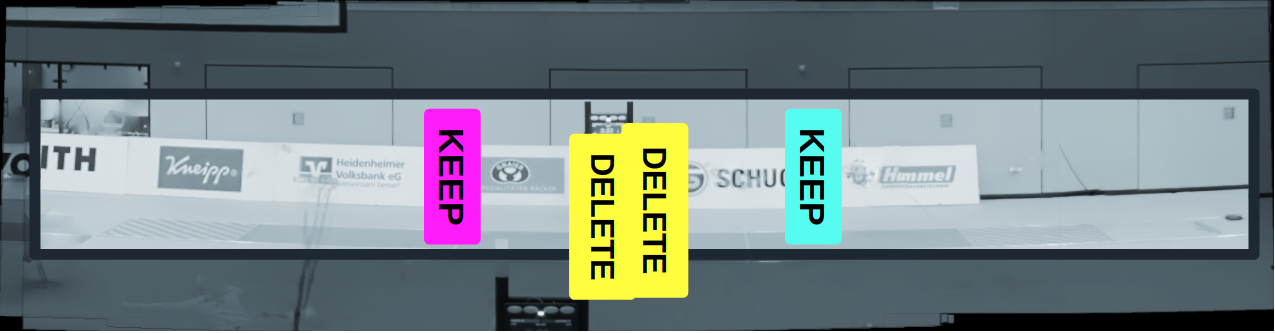
\includegraphics[width = \linewidth]{images/fencing/delete_panorama.png}}
% \subfloat[Overlay of the corresponding player in the unattended panorama]{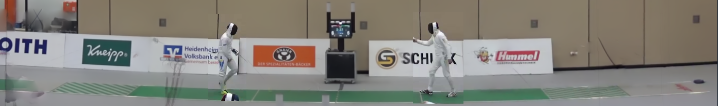
\includegraphics[width = \linewidth]{images/fencing/people_panorama.png}}
% \subfloat[Visualization of skeletal information of the corresponding player (posture estimation using Pif Paf)]{
\includegraphics[width = \linewidth]{images/fencing/skeleton_panorama.png}}
% \end{tabular}
% \caption{The process of extracting the skeletal and location information of the corresponding player from an unattended panorama}.
% \label{panos}
% \\end{figure}


% \subsection{Visualization and analysis of skeletal and positional information}.
% From the posture and positional information, clustering of action sequences and correlation with scoring situations can be analyzed to understand frequent plays in fencing and how players changed their playing style depending on the situation.


% %\subsubsection{analysis using clustering with mixed Gaussian model}}
% %\subsubsection{analysis with clustering}
% As an example application of the proposed framework, we perform clustering of skeletal information.
% The skeletal information is dimensionally compressed using PCA\cite{wold1987principal} and clustering is performed using the mixed Gaussian model\cite{bishop2006pattern}.
% The mixture Gaussian model can represent a Gaussian distribution with different parameters for each cluster.
% For the number of clusters, we use the minimum value of the Bayesian information criterion (BIC) \cite{jones2011bayesian}.
% The BIC is a measure of the negative log-likelihood with a constraint that the number of parameters should not be too large.
